\section{代码布局(Code Layout)}

\begin{frame}[fragile]
    \frametitle{什么是代码布局}
    指令连续地、有顺序地储存在内存中。LLVM中,这些优化过程抽象成控制流图中的基本块(Basic Block, BB)的排列方式。

    \begin{columns}
        \begin{column}{0.2\textwidth}
            \centering
            C Codes:
            \begin{lstlisting}
if (a <= b)
    c = 1;\end{lstlisting}
        \end{column}
        \begin{column}{0.5\textwidth}
            \begin{verbatim}
; a is in rax
; b is in rdx
; c is in rcx
cmp rax, rdx
ja .label
mov rcx, 1
.label:
            \end{verbatim}
        \end{column}
    \end{columns}
\end{frame}

\begin{frame}
    \frametitle{机器代码布局优化}
    基于机器相关的,代码布局的优化主要包含,基本块放置(Basic block placement)、基本块对齐(Basic block alignment)、冷热代码分离(Hot-Cold Splitting)\cite{bakhvalov-2019}.
    \begin{figure}
        \centering
        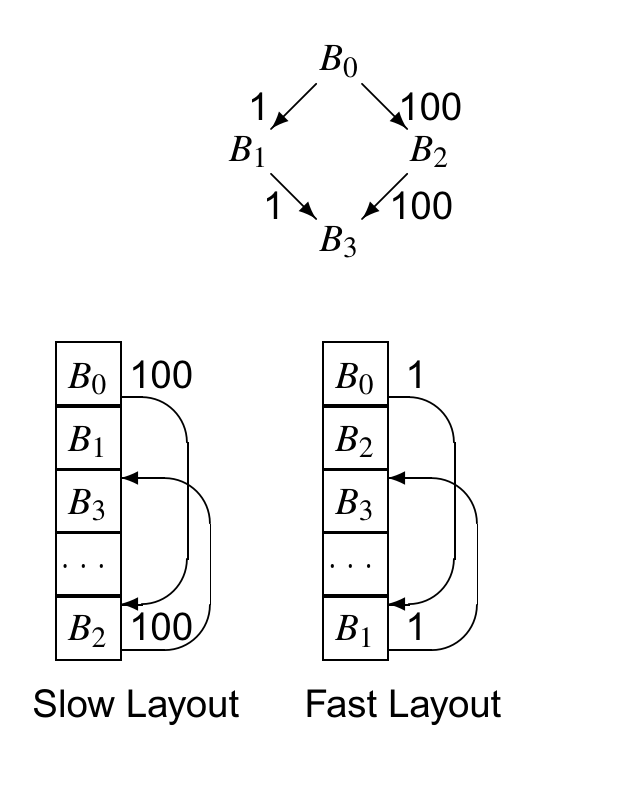
\includegraphics[width=0.31\textwidth]{images/layout_compare.png}
        \caption{两种不同布局的优劣\cite{cooper2011engineering}}
    \end{figure}

\end{frame}